
% LICENSE:
% Creative Commons Attribution-Sharealike 4.0 license (a.k.a. CC BY-SA) (#ccbysa).
% See the file LICENSE in this source distribution.

\documentclass[10pt,aspectratio=169]{beamer}
%% \documentclass[handout,10pt,aspectratio=169]{beamer}

\newcommand{\pitem}{\pause\item}

\newenvironment{colblock}[3]{%
  \setbeamercolor{block body}{#2}
  \setbeamercolor{block title}{#3}
  \begin{block}{#1}}{\end{block}}

%% Red Block with only Body
\newenvironment{AlternativeRBBlock}[0]{%
  \setbeamercolor{block body}{bg=red!20}
  \begin{block}{}}{\end{block}}

%% red block with only body
\newenvironment{rbblock}[0]{%
  \begin{colblock}{}{bg=red!20}{bg=green}}{\end{colblock}}


\setbeamersize{description width=0.35cm}

%% \usepackage[backend=biber,style=numeric-comp,sorting=none]{biblatex}
%% \addbibresource{2020-CS-PD.bib}

\setbeamertemplate{blocks}[rounded][shadow=true]
\setbeamercolor{block body alerted}{bg=alerted text.fg!10}
\setbeamercolor{block title alerted}{bg=alerted text.fg!20}
\setbeamercolor{block body}{bg=structure!10}
\setbeamercolor{block title}{bg=structure!20}
\setbeamercolor{block body example}{bg=green!10}
\setbeamercolor{block title example}{bg=green!20}

% add outline at the start of each new section

\usepackage{upquote,textcomp}   % get correct ascii quotes in verbatim
\usepackage{cclicenses}

% allow positioning of one block over another
\usepackage[absolute,overlay]{textpos}
% while debugging absolute positions, it can be useful to uncomment
% the next line
%% \usepackage[texcoord,grid,gridunit=mm,gridcolor=red!10,subgridcolor=green!10]{eso-pic}

\usepackage[24hr,iso]{datetime}
\renewcommand{\dateseparator}{-}

\usepackage{bookmark}
\usepackage{etoolbox}
\usepackage{relsize}

%% don't put those navigation buttons at the bottom of the slide -
%% they never really get used
\beamertemplatenavigationsymbolsempty

%% \logo{\includegraphics[height=1cm]{algorithm-design-manual.png}}

%% for source code listings
\usepackage[T1]{fontenc}
\usepackage{textcomp}
\usepackage{lmodern}
\usepackage{moresize}
\usepackage[procnames]{listings}
%% special instructions to make sure we can paste from pdf
\makeatletter
\def\addToLiterate#1{\edef\lst@literate{\unexpanded\expandafter{\lst@literate}\unexpanded{#1}}}
\lst@Key{add to literate}{}{\addToLiterate{#1}}
\makeatother

%% customization of listings
\usepackage{color}

%% colors for various parts of the syntax
\definecolor{mygreen}{rgb}{0,0.6,0}
\definecolor{mygray}{rgb}{0.5,0.5,0.5}
\definecolor{mymauve}{rgb}{0.58,0,0.82}
\lstset{commentstyle=\color{mygreen}}
\lstset{keywordstyle=\color{blue}}
\lstset{rulecolor=\color{black}}
\lstset{stringstyle=\color{mymauve}}

\lstset{framexleftmargin=5mm, frame=shadowbox, rulesepcolor=\color{gray!25}}
\lstset{breaklines=true}
\lstset{columns=fullflexible}
\lstset{keepspaces=true}
\lstset{showstringspaces=false}
\lstset{showspaces=false}
\lstset{extendedchars=false}
\lstset{literate={-}{-}1}
\lstset{upquote=true}
\lstset{add to literate={~}{\ttil}{1}}

\usepackage{graphicx}
\usepackage{tikz}
\usepackage{hyperref}
\usepackage{url}
\usepackage{media9}

\usepackage{smartdiagram}

\usetikzlibrary{calc,trees,positioning,arrows,chains,shapes.geometric,decorations.pathreplacing,decorations.pathmorphing,shapes,matrix,shapes.symbols}

\title{Entropy in Evolutionary Algorithms}
\subtitle{Statistical mechanics bearing insight into evolution}
\author{Lucas Blakeslee and Aengus McGuinness}
\subject{Optimization, Evolution, Genetic Algorithms}

\institute[SF High]{
  Santa Fe High School \\
  Institute for Computing in Research}
\date{2021-03-20 \\
  {\smaller[2] Last built \today{}T\currenttime } \\
  \smallskip
      {\smaller[4] (You may redistribute these slides with their \LaTeX\
        \vspace{-0.1cm}
        source code under the terms of the \\
        Creative Commons Attribution-ShareAlike 4.0 public license)}
}

\begin{document}

\section*{Frontmatter}

\begin{frame}
  \maketitle
\end{frame}

\section{Abstract}

\begin{frame}{Abstract}
	Genetic algorithms (GAs) are an optimization technique inspired by
	natural selection. GAs have yielded good results in certain practical
	problems, yet there is still more to be understood about their
	behavior on a theoretical level. One approach is to look at the
	evolutionary process from the point of view of statistical mechanics,
	and interpreting jumps in fitness as phase transitions. Toward this
	goal we examine the behavior of \emph{entropy} in a GA that optimizes
	a simple function.  We find that entropy increases as a new species
	diversifies, but its upper bound decreases with most phase
	transitions (which correspond to evolutionary steps).
\end{frame}

\begin{frame}{Introduction}
	\begin{itemize}
		\item Genetic Algorithms (GAs) are stochastic search algorithms that take inspiration from evolutionary processes. 
		\item Entropy is a generic term that means disorder. You can calculate it many different ways one method is shannonian information.
		\item We were motivated to do in depth analysis of genetic algorithms in order to understand their behavior better on a theoretical level.
		\item Schrödinger's book, "What is Life", sparked a modern wave of interest in the study of thermodynamics and evolution together.
	\end{itemize}
\end{frame}

\begin{frame}{Research Question}
		What happpens to entropy as an organism evolves over time? 
\end{frame}

\begin{frame}{Hypothesis}
	We hypothesized that entropy would gradually rise as small non-significant
	mutations occured, and that occasionally one highly beneficial mutation in
	an organism would cause entropy to rapidly decrease as that mutation was
	selected for and spreads throughout the population, and that entropy would then
	begin to rise again in a cyclical pattern. We hypothesized that if we're considering
	entropy to be the number of possible states an organism can be in, the
	upper bounds of the entropy would never reach levels they were previously at.
\end{frame}

\begin{frame}{Genetic Algorithms}
	In brief Genetic Algorithms attempt to find the maximum value of a
	function (called a fitness function).They do so by having a population of candidate values that take steps through the domain of that function.  The steps have a random	component, but the randomness is directed by a principle akin to	natural selection: when a population member has a high fitness value,	it is more likely to survive and breed new population members that share some of its characteristics.
	\begin{center}
		\smartdiagram[flow diagram:horizontal]{Population, Fitness Evaluation, Selection, Crossover, Mutation}
	\end{center}
\end{frame}

\begin{frame}{Punctuated Equilibrium}
      	\centering
      	      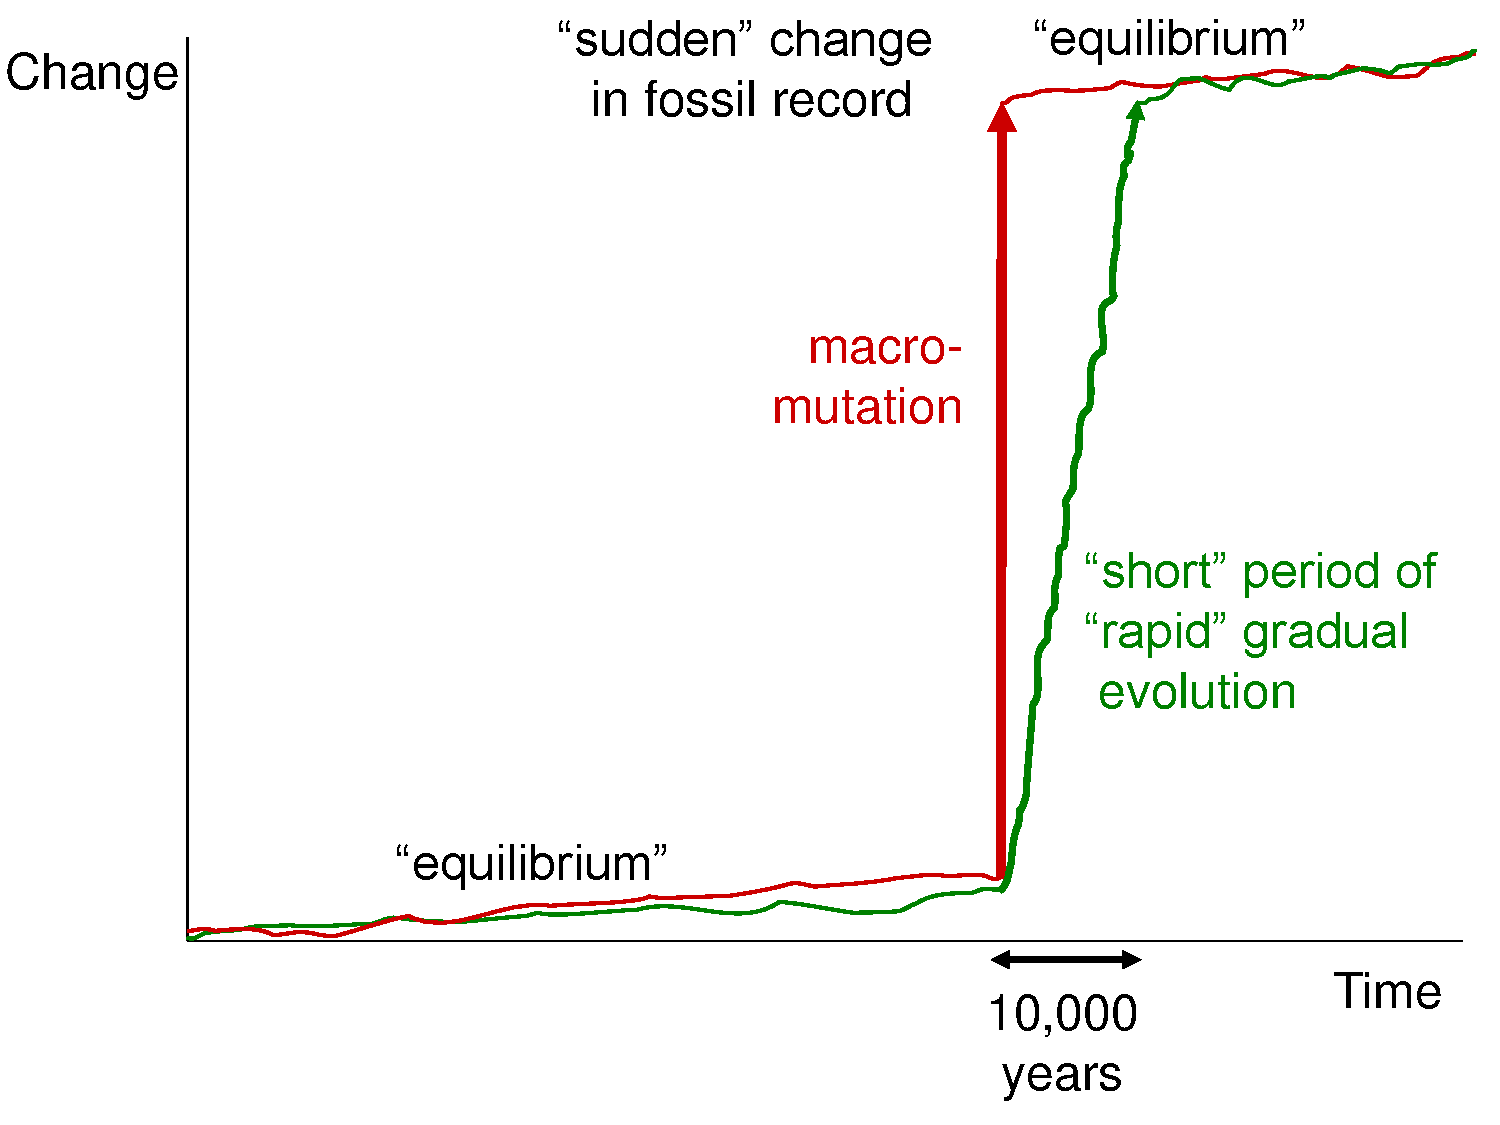
\includegraphics[width=0.75\textwidth]{Punctuated_Equilibrium.pdf}\\
      	      \tiny Ian Alexander, CC BY-SA 4.0 <https://creativecommons.org/licenses/by-sa/4.0>, via Wikimedia Commons
\end{frame}

\begin{frame}{Shannon Entropy}
		$
		Entropy \ H(X) = -\sum p(X)\log p(X)
		$
		\\
		"Amount of information" contained within a variable.
\end{frame}

\part{Part I, day 1}

\section{Experimentation}

\begin{frame}{Our GA}
	IEEE 754
\end{frame}

\begin{frame}{Pretty graphs}
  \begin{columns} % This creates a frame with multiple columns.
    % The first column will be 50% as wide as the width of text on the page.
    \begin{column}{0.4\textwidth}
      % Beamer doesn't like to display .eps files. This .png was
      % converted from .eps using Adobe Acrobat. The file graph1.png
      % should be in the same folder as the .tex file.
      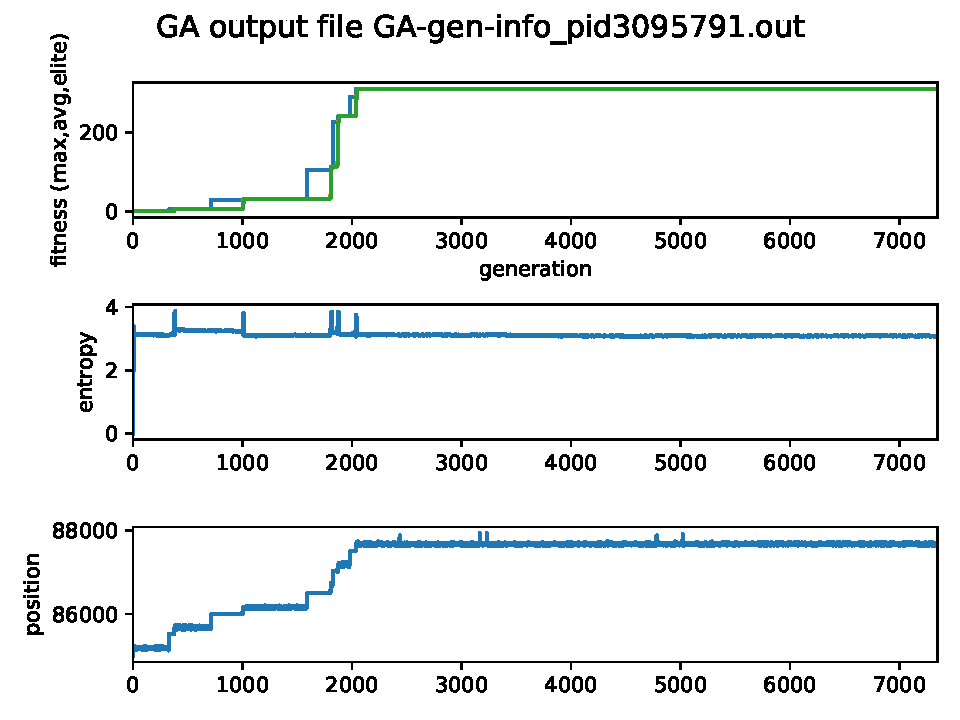
\includegraphics[width=\textwidth]{GA-gen-info_pid3095791.out.pdf}
                      {\tiny Woo hoo, graphs!\par}
    \end{column}

    \begin{column}{0.6\textwidth}
      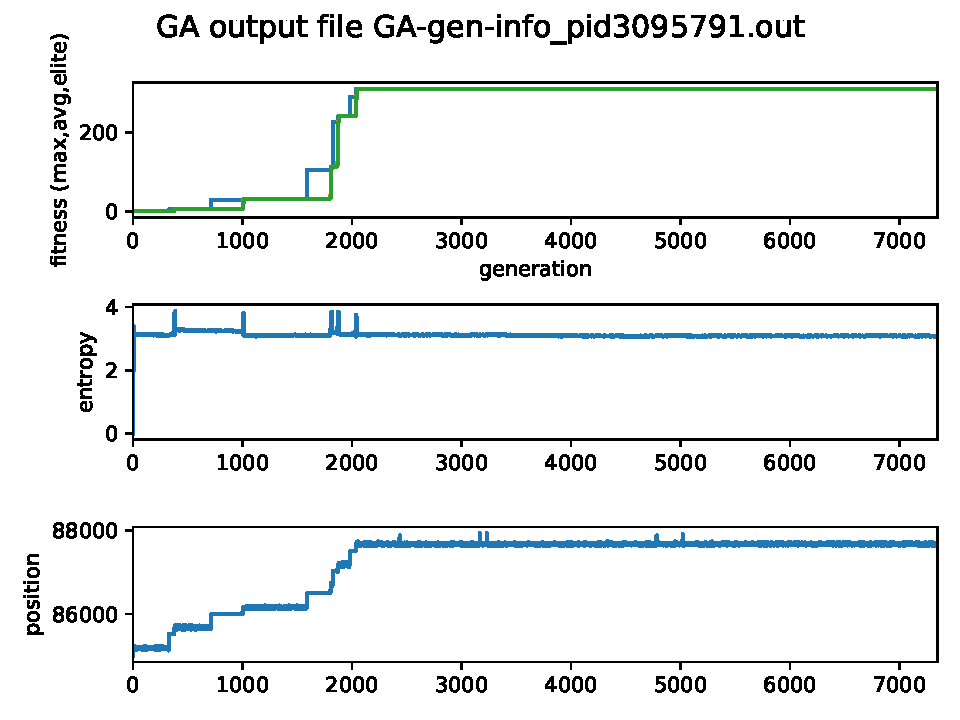
\includegraphics[width=0.75\textwidth]{GA-gen-info_pid3095791.out.pdf}\\
      				{\tiny The same one but in a different column!}
    \end{column}
  \end{columns}
\end{frame}



%% \input{curriculum}

%% \input{programming-languages}

%% \part{Part I, day 2}

%% \input{pedagogical}

%% \input{tools}

%% \input{bones-of-the-world}

%% %% \input{extras}

%% %% \input{references}

\end{document}
